%% ドキュメントクラスのロード jarticle クラス
%% onecolumn : 一段組み
%% a4j : A4サイズ,和文
%% fleqn : 数式は左揃え
\documentclass[11pt,twocolumn,a4paper, fleqn, uplatex]{ujarticle}

%% 使用パッケージの指定
%% graphicx : 図の使用
%% fancyhdr : ヘッダ設定
%% lastpage : ページ番号出力マクロ
\usepackage[dvipdfmx]{graphicx}
\usepackage{fancyhdr}
\usepackage{lastpage}
\usepackage{listings, jlisting}
\usepackage{bm}
\usepackage{mathptmx}
\usepackage{amsmath}
\usepackage{amsfonts}
\usepackage{amsmath}
\usepackage[subrefformat=parens]{subcaption}
\usepackage{geometry}

\lstset{
  numbers=left,
  numbersep=-10pt,
  columns=l
}
%ページの余白設定--------------------------------------------------
\geometry{left=15mm, right=15mm, bottom=20mm}

%自作コマンド--------------------------------------------------
%% 独自マクロ タイトルスタイルの変更
\makeatletter
\let\@oldmaketitle=\@maketitle
\def\@maketitle{
  \vskip -3zh
  \@oldmaketitle
  %\vspace*{-0.8cm}
}
\makeatother

%% 参照
\def\figref#1{図\ref{#1}}
\def\tblref#1{表\ref{#1}}
\def\eqref#1{式(\ref{#1})}
%----------------------------------------------------------------

%% ページのレイアウト指定
\setlength{\textheight}{242mm}
\setlength{\mathindent}{1zw}
\setlength{\headheight}{15.0pt}
\setlength{\voffset}{-1cm}

%% ヘッダスタイルの適用
\pagestyle{fancy}
\lhead{ 輪講 \today{}}
\chead{}
\rhead{}
\lfoot{}
\cfoot{\thepage}
\rfoot{}
\renewcommand\headrulewidth{0.4pt}
\renewcommand\footrulewidth{0pt}


\title{
  {\Large{\bf タイトル }}
}
\author{\bf{XXXX XXX}\\
}
\date{}

%%----- ここから論文本体 ---------------------------------------
\begin{document}
\maketitle
\section{はじめに}
資料作成に関して,いろいろ書式とか慣習があったりします.rocky研だと厳し目に指導されますので,詳しくはrocky研のサイトの論文執筆にあたってを見てください.
もしかして,rocky研の人じゃないですか?ぜひテンプレートをつかっていただきたいところですが,分野やお家ごとに慣習が異なると思うので,参考程度に使ってください.
\LaTeX ってコマンド覚えるの大変ですけど,慣れると綺麗な資料が作れると思っているので一緒にがんばりましょう.

\section{数式}\label{sec1}
詳しくは,\LaTeX の解説情報がインターネット世界にたくさんあるので,バージョンだけ注意して解説を見てもらったほうがいいと思ってます.
個々では,このテンプレートを使うときに便利だよってやつを載せています.

\begin{equation}
    \int^{b}_{a}f(x)dx = \int^{c}_{a}f(x)dx + \int^{b}_{c}f(x)dx
    \label{eq:sample}
\end{equation}

行列とか,ベクトルとか書きたい時は,$\bm{P}$, $\bm{a}$ みたいにかく.
数式なんだけど,イタリックにしたくない時はmathrmを使います.例えば,転置行列を表記するときの記号Tは,こんな感じ.$\bm{A}^{\mathrm{T}}$
それから,花文字使いたいなって時は,こうしましょう $\mathcal{W}$.

最適化問題の定式化なんかは,数式環境で更にaligned環境を使ってこうやって書きます.
\[
\begin{aligned}
    & \underset{\bm{x}} {\text{min}} && \sum_{i=1}^{n} \lambda_i x_i  \\ &&& \bm{x} = (x_1 \cdots x_n)^{\mathrm{T}},\lambda_i \in \mathbb{R}, i \in \{1,..., n\} \\\
&\text{subject to} && \sum_{i=1}^{n/2} x_i = \mathrm{A} &&& \\
&                  &&  \sum_{i=n/2+1}^{n} x_i = \mathrm{B}\\ &&& \\
    &                  &&  \mathrm{"条件式を書く"}  \\&&&  \mathrm{変数の条件を書く} \\
&                  && \mathrm{\bm{p}}_3^{\mathrm{T}} \ge 0 \\ &&&  \forall i \in \{1, ..., n_c\}
\end{aligned}
\]
\section{図,表を入れる}\label{sec2}
図を入れるときはこんな.
ただし,グラフはないよとは全く関係ありません.
\begin{figure}[htbp]
    \centering
    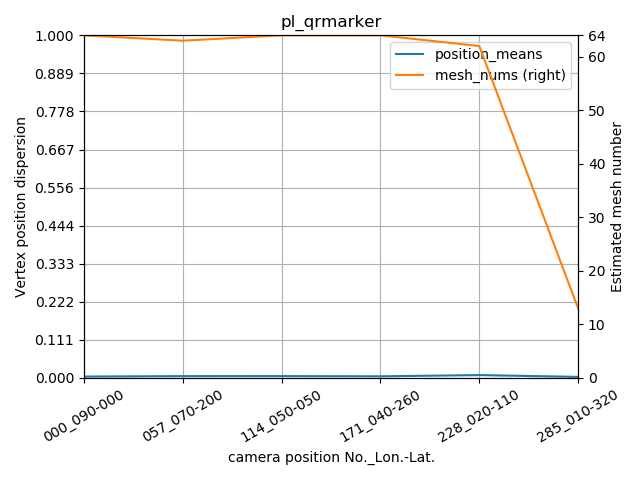
\includegraphics[width=0.7\linewidth]{img/fig.png}
    \caption{画像いっこ}
    \label{fig:label1}
\end{figure}

画像を並べたいって時はminipage環境を改行して表記する
\begin{figure}[htbp]
  \begin{minipage}[t]{\hsize}
    \centering
    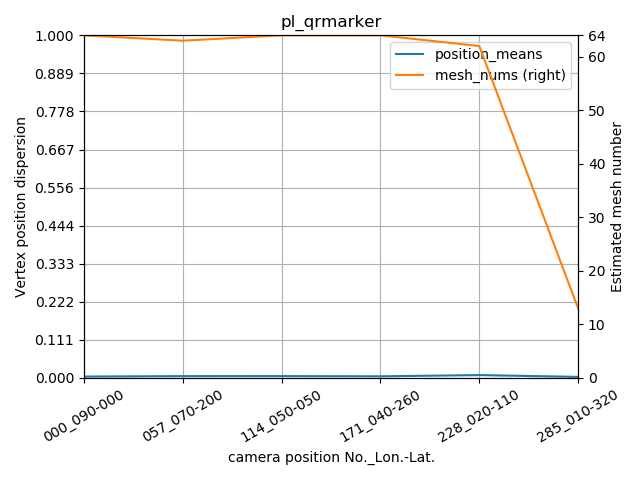
\includegraphics[width=0.6\linewidth]{img/fig.png}
    \subcaption{画像ひとつめ}
    \label{fig:niko1}
  \end{minipage}
    \\
  \begin{minipage}[t]{\hsize}
    \centering
    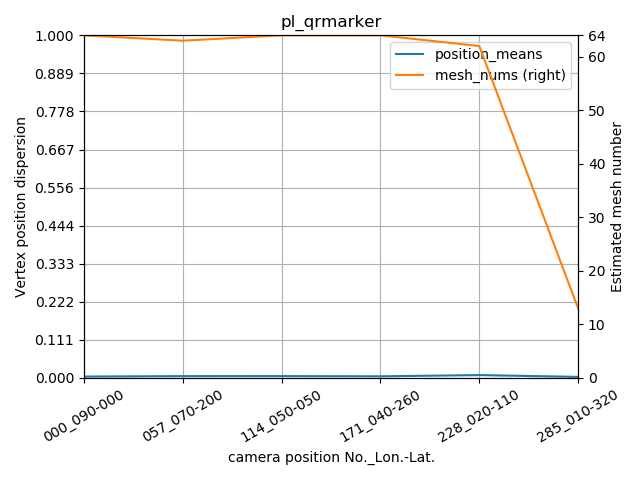
\includegraphics[width=0.6\linewidth]{img/fig.png}
    \subcaption{ふたつめ}
    \label{fig:niko1}
  \end{minipage}
 \caption{まとめて画像を表示する}
\end{figure}

いや,幅小さくて画像がかえって見難い!そんな時はカラムをぶちぬいてやりましょう.
figure環境のうしろに*をつけてやるだけです.
\begin{figure*}[htbp]
    \centering
    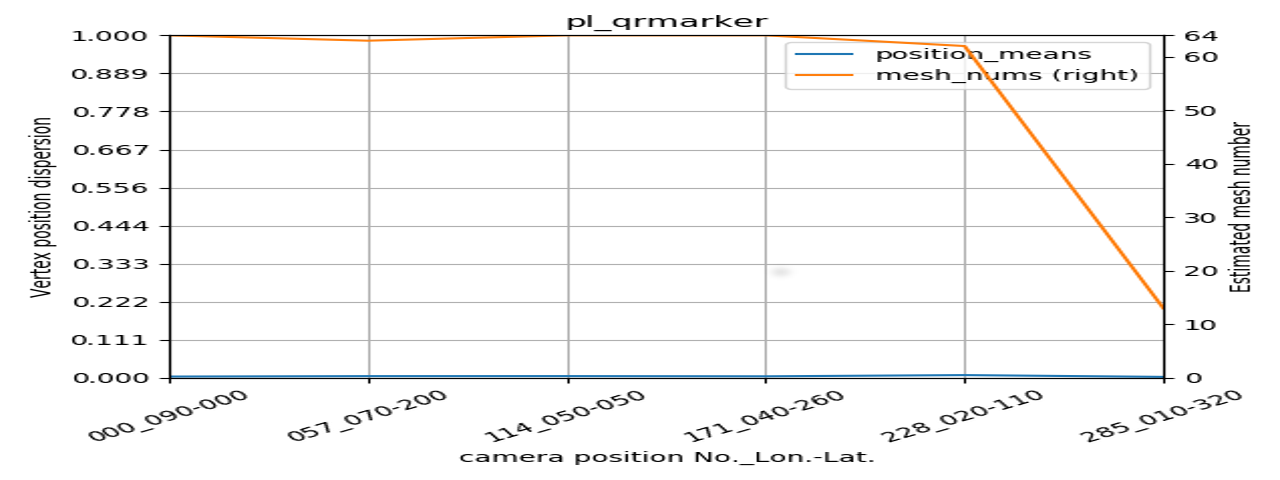
\includegraphics[width=150mm]{img/fig-buchi.png}
    \caption{ぶちぬいてやったぜ}
    \label{fig:buchi}
\end{figure*}

表を入れたいって時はこうします.tablar環境で列と各列の配置を定義します.各行の要素は\&でつなぎます
列の配置はl:left,r:right,c:centerの頭文字です.縦棒|は表の縦線を定義してます.二重線にしたいときは||とすればOKです.
横線は$\backslash$hlineです.
\begin{table}[htb]
  \begin{tabular}{|c||r|l|} \hline
    中央よせ & みぎよせ & ひだりよせ \\ \hline \hline
    例 & 2.261 & 数字は右寄せがいい  \\ \hline
  \end{tabular}
  \caption{表の例}
  \label{tbl:ex}
\end{table}

\subsubsection{相互参照付けたい}
表とか,式とか,図とかを出したら参照して文章中に説明しないといけないです.
そんな時にふつうは$\backslash$ref\{xxx\}なんてlabelのxxxを参照するのですが,
いつも図xx,式(a)とかやるのが面倒で最悪忘れます.そんな時に役立つマクロをつけてあります.
プリアンブルにマクロを定義しています.詳しくはGoogleで調べて貰えばいいと思います.
文章中で参照したくなったら,このテンプレートではこうやってつかってください.
\begin{description}
    \item[図を参照したい時]\mbox{}\\ 
        $\backslash$figref\{xxx\}とします.実際にはこんな感じ,\figref{fig:niko1}によると,カラムスタイルの時の画像のぶち抜いた時の状態を示している.
    \item[数式を示したい]\mbox{}\\
        $\backslash$eqref\{xxx\}とします.実際にはこんな感じ,\eqref{eq:sample}は積分の式.マクロなら,カッコ付きの参照を出力してくれる!
    \item[表を参照したい時]\mbox{}\\
        図と同じ,$\backslash$tblref\{xxx\}とします.\tblref{tbl:ex}
\end{description}

\section{参考文献どうする?}
参考文献のスタイルについての細かいルールは,やはり,詳しくはrocky研のサイトの論文執筆にあたってを見てください.
ただし,このテンプレートではBiblatexというツールを利用しています.このツールに関する解説もGoogleで調べてください.
Biblatexは***.libというテキストベースの参考文献リストを参照して自動的に予め決めたスタイルにしたがって,参考文献の参照および参考文献リストを記述してくれるすぐれものです.
このテンプレートでは,mainbib.libという参考文献リストファイルに参考文献をまとめています.
そして,以下に書いている$\backslash$bibliography{mainbib}部分で参考文献リストファイルを指定しています.
文献の参照方法は文献\cite{latex2e}を参照するといいと思います.\LaTeX 全般の使い方が書いてあります.


%% 参考文献
\bibliographystyle{sieicej}
\bibliography{library}%bibTexのファイル名

\end{document}
